\documentclass{article}

\usepackage[a4paper, margin=0.5in]{geometry}
\usepackage{hyperref}
\usepackage{graphicx}
\usepackage{enumitem}
\usepackage{listings}
\usepackage{xcolor}
\usepackage{fancyvrb}
\usepackage{longtable}
\usepackage{wrapfig}
\usepackage{booktabs}
\usepackage{mdframed}
\usepackage{lmodern} % For better font rendering
\usepackage{titlesec} % titleformat

\definecolor{codebg}{rgb}{0.95,0.95,0.95}

\lstset{
    backgroundcolor=\color{codebg},
    basicstyle=\ttfamily\small,
    frame=single,
    breaklines=true
}

% setup something below subsubsection
\setcounter{secnumdepth}{4}
\setcounter{tocdepth}{4}

\titleclass{\subsubsubsection}{straight}[\subsection]

\newcounter{subsubsubsection}[subsubsection]
\renewcommand\thesubsubsubsection{\thesubsubsection.\arabic{subsubsubsection}}
\renewcommand\theparagraph{\thesubsubsubsection.\arabic{paragraph}} % optional; useful if paragraphs are to be numbered

\titleformat{\subsubsubsection}
  {\normalfont\normalsize\bfseries}{\thesubsubsubsection}{1em}{}
\titlespacing*{\subsubsubsection}
{0pt}{3.25ex plus 1ex minus .2ex}{1.5ex plus .2ex}

\titleformat{\paragraph}
{\normalfont\normalsize\bfseries}{\theparagraph}{1em}{}
\titlespacing*{\paragraph}
{0pt}{3ex plus 1ex minus .3ex}{1.5ex plus .2ex}

\makeatletter
\renewcommand\subparagraph{\@startsection{subparagraph}{6}{\parindent}%
  {3.25ex \@plus1ex \@minus .2ex}%
  {-1em}%
  {\normalfont\normalsize\bfseries}}
\def\toclevel@subsubsubsection{4}
\def\toclevel@paragraph{5}
%\def\toclevel@paragraph{6}
\def\toclevel@subparagraph{6}
\def\l@subsubsubsection{\@dottedtocline{4}{7em}{4em}}
\def\l@paragraph{\@dottedtocline{5}{10em}{5em}}
\def\l@subparagraph{\@dottedtocline{6}{14em}{6em}}
\makeatother

% end of paragraph setup

\begin{document}

\section{Snippets}

\subsection{Find all image textures path}
\begin{lstlisting}[language=Python]
for img in bpy.data.images:
    print(img.name, ":", img.filepath)
\end{lstlisting}

\subsection{Manipulate selected objects}
\begin{lstlisting}[language=Python]
for obj in bpy.context.selected_objects:
    obj.rotation_euler.x += 1.5708  # Rotate 90 degrees (π/2) on X-axis
\end{lstlisting}

\section{Shortcuts}

\subsection{Selection \& Navigation}

\begin{longtable}{ll}
    \toprule
    \textbf{Shortcut}    & \textbf{Effect}                                                \\
    \midrule
    \endhead
    \bottomrule
    \endfoot

    \textbf{Ctrl + `}    & Hide/Show gizmos                                               \\
    \textbf{Tab}         & Toggle between Object Mode and Edit Mode                       \\
    \textbf{A}           & Select all                                                     \\
    \textbf{Alt + A}     & Deselect all                                                   \\
    \textbf{L}           & Select linked geometry (hover over a part and press L)         \\
    \textbf{Ctrl + L}    & Select all linked geometry (based on selection)                \\
    \textbf{B}           & Box select                                                     \\
    \textbf{C}           & Circle select                                                  \\
    \textbf{Shift + G}   & Select similar (choose criteria like area, shape, or material) \\
    \textbf{Alt + RMB}   & Loop select                                                    \\
    \textbf{Shift + RMB} & Ring select                                                    \\
\end{longtable}

\subsection{Transformations}

\begin{longtable}{ll}
    \toprule
    \textbf{Shortcut}                                         & \textbf{Effect}                                                    \\
    \midrule
    \endhead
    \bottomrule
    \endfoot

    \textbf{Ctrl + `}                                         & Hide/Show gizmos                                                   \\
    \textbf{Tab}                                              & Toggle between Object Mode and Edit Mode                           \\
    \textbf{A}                                                & Select all                                                         \\
    \textbf{Alt + A}                                          & Deselect all                                                       \\
    \textbf{L}                                                & Select linked geometry (hover over a part and press L)             \\
    \textbf{Ctrl + L}                                         & Select all linked geometry (based on selection)                    \\
    \textbf{B}                                                & Box select                                                         \\
    \textbf{C}                                                & Circle select                                                      \\
    \textbf{Shift + G}                                        & Select similar (choose criteria like area, shape, or material)     \\
    \textbf{Alt + RMB}                                        & Loop select                                                        \\
    \textbf{Shift + RMB}                                      & Ring select                                                        \\
    \midrule
    \textbf{G}                                                & Grab (move)                                                        \\
    \textbf{R}                                                & Rotate                                                             \\
    \textbf{S}                                                & Scale                                                              \\
    \textbf{X / Y / Z}                                        & Constrain movement to an axis (e.g., G + X moves along the X-axis) \\
    \textbf{Shift + X / Y / Z}                                & Move along the other two axes (exclude one axis)                   \\
    \textbf{Ctrl + A}                                         & Apply transformations (use in Object Mode)                         \\
    \midrule
    \textbf{Ctrl + Tab} (or \textbf{1, 2, 3} in Blender 2.8+) & Switch between Vertex, Edge, and Face selection                    \\
    \textbf{Ctrl + E}                                         & Edge menu (Bevel, Mark Seam, etc.)                                 \\
    \textbf{Ctrl + B}                                         & Bevel (works for edges and vertices)                               \\
    \textbf{Shift + Ctrl + B}                                 & Vertex bevel                                                       \\
    \textbf{F}                                                & Fill (creates a face between selected vertices/edges)              \\
    \textbf{Alt + Left Click}                                 & Select edge loop                                                   \\
    \textbf{Shift + Alt + Left Click}                         & Select multiple edge loops                                         \\
    \midrule
    \textbf{Ctrl + R}                                         & Loop cut (scroll mouse wheel to increase cuts)                     \\
    \textbf{K}                                                & Knife tool (click to cut, Enter to confirm)                        \\
    \textbf{Shift + R}                                        & Repeat last action                                                 \\
    \textbf{Ctrl + Shift + B}                                 & Chamfer/Bevel vertices                                             \\
\end{longtable}

\subsection{Extrude, Inset \& Merge}

\begin{longtable}{ll}
    \toprule
    \textbf{Shortcut} & \textbf{Effect}                                               \\
    \midrule
    \endhead
    \bottomrule
    \endfoot

    \textbf{E}        & Extrude                                                       \\
    \textbf{I}        & Inset faces                                                   \\
    \textbf{M}        & Merge vertices (choose options like "At Center" or "At Last") \\
    \textbf{Alt + M}  & Older version of merge (pre-2.8)                              \\
\end{longtable}

\subsection{Proportional Editing \& Smoothing}

\begin{longtable}{ll}
    \toprule
    \textbf{Shortcut}         & \textbf{Effect}                                  \\
    \midrule
    \endhead
    \bottomrule
    \endfoot

    \textbf{O}                & Toggle Proportional Editing                      \\
    \textbf{Shift + O}        & Change proportional falloff type                 \\
    \textbf{Ctrl + Shift + B} & Bevel vertices                                   \\
    \textbf{Shift + S}        & Snap menu (snap selection to grid, cursor, etc.) \\
    \textbf{U}                & Unwrap UV (when in UV Editing)                   \\
    \textbf{Ctrl + T}         & Triangulate faces                                \\
    \textbf{Alt + J}          & Convert tris to quads                            \\
\end{longtable}

\subsection{Miscellaneous}

\begin{longtable}{ll}
    \toprule
    \textbf{Shortcut}  & \textbf{Effect}                      \\
    \midrule
    \endhead
    \bottomrule
    \endfoot

    \textbf{H}         & Hide selection                       \\
    \textbf{Alt + H}   & Unhide all                           \\
    \textbf{Shift + H} & Hide everything except selection     \\
    \textbf{P}         & Separate selection into a new object \\
    \textbf{Ctrl + J}  & Join selected objects                \\
\end{longtable}

\begin{itemize}[topsep=0pt, noitemsep]
    \item Edit mode UV tools: press U
    \item Edge slide tool: in edit mode, with a vertex selected, press Grab (G) twice
    \item Triplanap projection: \href{https://www.youtube.com/watch?v=KV_hgeQdCXk}{https://www.youtube.com/watch?v=KV\_hgeQdCXk}
    \item Baking: \href{https://www.youtube.com/watch?v=sOvRr_D8ZpU}{https://www.youtube.com/watch?v=sOvRr\_D8ZpU}
\end{itemize}

\section{Pivot to Cursor}
Press \textbf{Shift + Right Click} to place the 3D Cursor manually.  Or use \textbf{Shift + S} → "Cursor to Selected" to place it at the selection.\par
Instead, to change the pivot point to cursor, do the following:
\begin{itemize}[topsep=0pt, noitemsep]
    \item In \textit{Object Mode}, go to the top-center of the viewport (next to the selection mode dropdown) where the pivot point options are.
    \item Click on the Pivot Point dropdown (it's an icon that usually shows a circle with a dot in the center).
    \item Select 3D Cursor from the list of pivot options.
\end{itemize}
Alternatively:
\begin{itemize}[topsep=0pt, noitemsep]
    \item Period key (.) to open the pivot point menu and choose 3D Cursor.
    \item Perm
    \item Object - Set Origin
\end{itemize}

\section{Sharing: Asset Browser}
Video Reference: \href{https://www.youtube.com/watch?v=cbzBt60dhY8}{https://www.youtube.com/watch?v=cbzBt60dhY8}\\

\section{Animations: Docs Summary}
These notes about animations in Blender are made by summarizing the \href{https://docs.blender.org/manual/en/4.3/animation/introduction.html}{Blender 4.3 Docs}.

\subsection{Introduction}

Animation = Transforming an object or changing its shape over time. More generally, any property about a blender object can be animated. \\
Animation is typically achieved by employing \textit{Keyframes} (more on that later) \\\\
Any property in the \textit{Properties Editor} has a \textit{State Color}

\begin{center}
    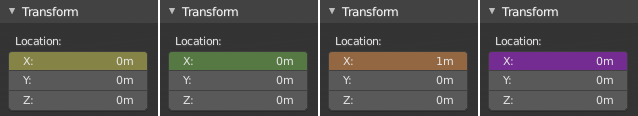
\includegraphics[width=0.7\textwidth]{blender_docs_images/animation_introduction_state-colors.png}
\end{center}

\begin{longtable}{cl}
    \toprule
    \textbf{Color} & \textbf{Meaning}                 \\
    \midrule
    \endhead
    \bottomrule
    \endfoot

    Gray           & Not animated                     \\
    Yellow         & Changed from the current frame   \\
    Green          & Keyframed on a different frame   \\
    Orange         & Changed from the keyframed value \\
    Purple         & Controlled by a \textit{Driver}  \\
\end{longtable}

\subsubsection{Rigging}

Rigging = adding controls handles to animate an object. Blender offers the following feature to rig a model
\begin{longtable}{p{0.2\textwidth}p{0.7\textwidth}}
    \toprule
    \textbf{Rigging Method}   & \textbf{Brief}                                                                                                                                                                                                                                                                                                         \\
    \midrule
    \endhead
    \bottomrule
    \endfoot

    \textbf{Armatures}        & A Hierarchy of Joints associated with a mesh. Each joint has a *weight* [0.0, 1.0] for each vertex of the aforementioned mesh (can be painted). Transforming a joint will influence all vertices whose weight for that particular joint is greater than 0. This technique is called *Skeletal Animation* (more later). \\
    \textbf{Constraints}      & Control the kind of motion the rig is allowed to perform. They are found under \textit{Properties Editor}, tab "Constraints" (more later).                                                                                                                                                                             \\
    \textbf{Object Modifiers} & Mesh deformation through modifiers. We are interested in \href{https://docs.blender.org/manual/en/4.3/modeling/modifiers/deform/index.html}{Deformations} and \href{https://docs.blender.org/manual/en/4.3/modeling/modifiers/physics/index.html}{Physics} (more later).                                               \\
    \textbf{Shape Keys}       & Commonly called textit{blendshape}, meaning having different copies of a mesh (same topology, same UV, same *everything*). Example: different facial expressions that blend over time with \textit{Keyframing} (more later).                                                                                           \\
    \textbf{Drivers}          & Mechanisms to control multiple properties at once and make some properties automatically update when others change (more later).                                                                                                                                                                                       \\
\end{longtable}

\subsection{Keyframes}

\subsubsection{Relevant Shortcuts}
\textbf{With a property/object Selected:}
\begin{longtable}{ll}
    \toprule
    \textbf{Shortcut}  & \textbf{Effect}                                \\
    \midrule
    \endhead
    \bottomrule
    \endfoot

    \textbf{I}         & Insert Keyframe (brings up keyframe menu)      \\
    \textbf{Alt + I}   & Delete Keyframe                                \\
    \textbf{Shift + I} & Insert Keyframe for all properties             \\
    \textbf{Ctrl + I}  & Add keyframe to active keying set              \\
    \textbf{Alt + S}   & Reset Scale (useful when animating transforms) \\
    \textbf{Alt + R}   & Reset Rotation                                 \\
    \textbf{Alt + G}   & Reset Location                                 \\
\end{longtable}
\textbf{Inside \textit{Graph Editor} or \textit{Dope Sheet Editor}}
\begin{longtable}{ll}
    \toprule
    \textbf{Shortcut}             & \textbf{Effect}                                             \\
    \midrule
    \endhead
    \bottomrule
    \endfoot

    \textbf{G}                    & Move keyframe(s)                                            \\
    \textbf{S}                    & Scale keyframe(s)                                           \\
    \textbf{R}                    & Rotate keyframe handle (in Graph Editor)                    \\
    \textbf{Shift + D}            & Duplicate keyframe(s)                                       \\
    \textbf{X} or \textbf{Delete} & Delete keyframe(s)                                          \\
    \textbf{E}                    & Extrapolate (Graph Editor)                                  \\
    \textbf{T}                    & Set Keyframe Interpolation (Linear, Bezier, Constant, etc.) \\
    \textbf{V}                    & Set Keyframe Handle Type (Vector, Aligned, etc.)            \\
    \textbf{Ctrl + C}             & Copy Keyframe                                               \\
    \textbf{Ctrl + V}             & Paste Keyframe                                              \\
\end{longtable}

\textbf{Playback Shortcuts}
\begin{longtable}{ll}
    \toprule
    \textbf{Shortcut}                   & \textbf{Effect}                                               \\
    \midrule
    \endhead
    \bottomrule
    \endfoot

    \textbf{Spacebar}                   & Play/Pause animation                                          \\
    \textbf{Shift + Left Arrow}         & Jump to \textbf{start frame}                                  \\
    \textbf{Shift + Right Arrow}        & Jump to \textbf{end frame}                                    \\
    \textbf{Left Arrow}                 & Move \textbf{one frame backward}                              \\
    \textbf{Right Arrow}                & Move \textbf{one frame forward}                               \\
    \textbf{Up Arrow}                   & Move to \textbf{next keyframe}                                \\
    \textbf{Down Arrow}                 & Move to \textbf{previous keyframe}                            \\
    \textbf{Shift + Ctrl + Spacebar}    & Play animation in \textbf{reverse}                            \\
    \textbf{Home}                       & Zoom to fit all keyframes in \textbf{Graph Editor/Dope Sheet} \\
    \textbf{Ctrl + Middle Mouse Scroll} & Zoom in/out in Timeline/Graph Editor                          \\
\end{longtable}
When you set a keyframe on a simple static mesh, like a cube. \\ (in the Viewport, object mode, Ctrl + A -> Mesh -> Cube). If
\begin{itemize}[topsep=0pt, noitemsep]
    \item You press \textbf{I}, then all the transform properties are saved in the current frame as a keyframe (see in \textit{Dope Sheet Editor})
    \item If you want only a part of the default properties to be saved, then you can set them manually by clicking the \textit{Animate Property} handle to
          the right of the property in the \textit{Properties Editor}
          \begin{center}
              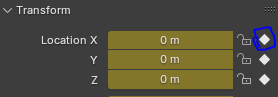
\includegraphics[width=0.4\textwidth]{blender_docs_images/my_properties_animate_handle.png}
          \end{center}
\end{itemize}

\subsubsection{Introduction}
A \textit{Keyframe} is a marker of time which stores the value of the selected property.\\
The purpose of a keyframe is to save the value of a property in a given instance of "time" (on a rendered frame. Physical elapsed time depends on the FPS of the animation).\par

An overview of all the existing keyframe in your animation can be seen in the \textit{Playback Editor}. To get the full information about existing keyframes (ie. to which
object they refer to and which property they alter/set, use the \textit{Dope Sheet Editor}).
\begin{center}
    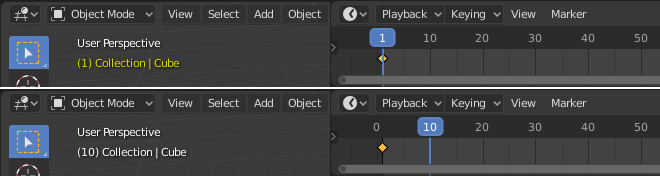
\includegraphics[width=0.7\textwidth]{blender_docs_images/animation_keyframes_introduction_visualization.png}
\end{center}
\begin{mdframed}[linewidth=2pt, linecolor=gray, roundcorner=1pt, innermargin=2pt, outermargin=2pt]
    \textbf{\Large Quick Experiment: Keyframe Visualization} \\[6pt]
    \textbf{File:} \texttt{01\_Keyframes\_Intro-Moving\_Cube.blend} \\[6pt]

    \begin{enumerate}[topsep=0pt, noitemsep]
        \item Create an empty Blender scene with a cube and check FPS \\
              (\textit{Properties Editor} $\rightarrow$ Output $\rightarrow$ Frame Rate).
        \item Select its position from the \textit{Properties Editor} and set a keyframe (\textbf{I} to keyframe the transform).
        \item Move to another keyframe inside \textit{Dope Sheet Editor} or \textit{Playback Editor}.
        \item Freely transform your cube and then set a keyframe. \\
              \textbf{Note:} It's imperative that you first move to another place in the timeline and then manipulate your object, otherwise it won't work!
        \item Go back to the start of the timeline (\textbf{Shift + Left Arrow}) and play the animation (\textbf{Spacebar}).
    \end{enumerate}

    \textit{Keep this example for the next section on Interpolation.}
\end{mdframed}

\paragraph{Interpolation}
When you set two keyframes on the same property, its value changes over the span of frames inbetween the two keyframes with \textit{Interpolated Values}, ie values computed using
a matematical formula. In particular, such formula is defined by an \href{https://docs.blender.org/manual/en/4.3/editors/graph_editor/fcurves/introduction.html}{\textit{F-Curve}},
manipulated in the \textit{Graph Editor}.
\begin{center}
    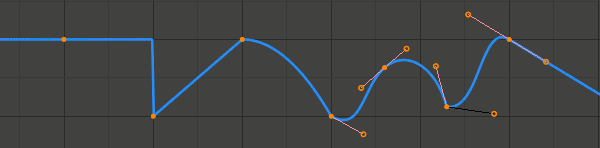
\includegraphics[width=0.7\textwidth]{blender_docs_images/animation_keyframes_introduction_curves.png}
\end{center}

There is 1 curve for each animated property in the \textit{Dope Sheet Editor}. The main setting is the \textit{Interpolation} Type, which appears in the \textit{Graph Editor} inside the
\textit{F-Curve} Tab. \textbf{Interpolation Modes:}\footnote{All the settings inside the \textit{F-Curve} Tab affect the keyframes selected}
\begin{itemize}[topsep=0pt, noitemsep]
    \item Bezier Curve
    \item Linear
    \item Constant
\end{itemize}
\begin{center}
    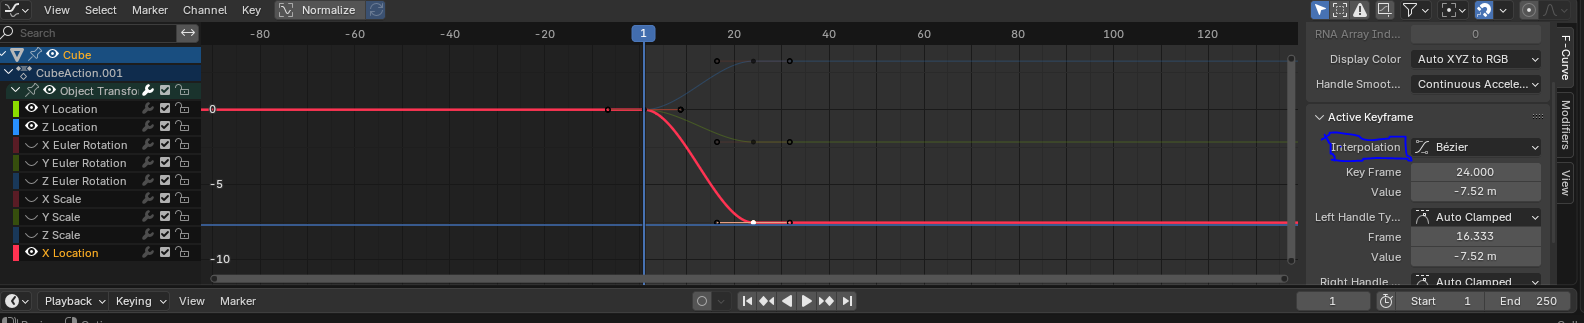
\includegraphics[width=0.9\textwidth]{blender_docs_images/my_graph_editor_interpolation_mode.png}
\end{center}
While what happens during the transition between a keyframe and the next one is defined by the \textit{Interpolation} Mode, What happens outside the "Keyframed Range"
(before the first keyframe and after the last keyframe) is defined by the \textit{Extrapolation Mode}.\par
\textit{Extrapolation Mode} is found under \mbox{"\textit{Graph Editor}/Channel/Extrapolation Mode"} or with shortcut \textbf{Shift + E} (\textit{Graph Editor} Selected)
The following are the available \textbf{Extrapolation Modes:}\footnote{Extrapolation Mode affects all \textit{F-Curves} selected}
\begin{itemize}[topsep=0pt, noitemsep]
    \item Constant: Continue in a straight horizontal line
    \item Linear: Continue in a straight line keeping the slope
    \item Make Cyclic: Repeat the curve
    \item Clear Cyclic: Removes Cycles Modifier
\end{itemize}

The settings to manipulate Curve Handles (placed on the F-Curve on the keyframe positions) depend on the Interpolation Type. A common setting among them all is the
\textit{Auto Handle Smoothing}, which can be either \textit{None} or \textit{Continuous Acceleration}.\par
When not \textit{None}, edits to a handle are propagated in the near handles (similiar to proportional editing) to keep the F-Curve as smooth as possible.
\begin{mdframed}[linewidth=2pt, linecolor=gray, roundcorner=1pt, innermargin=2pt, outermargin=2pt]
    \textbf{\Large Quick Experiment: Interpolation and Extrapolation: "Cyclic Overshoot"} \\[6pt]
    \textbf{File:} \texttt{02\_Keyframes\_Interpolation-Moving\_Cube\_Custom\_Interpolation.blend} \\[6pt]

    \begin{enumerate}[topsep=0pt, noitemsep]
        \item Open the cube example you produced from the previous experiment
        \item Open the \textit{Graph Editor} and select a "Location" Curve (the one with the bigger displacement in the Vertical axis)
        \item Play around with the 2 Handles freely. Example: Use the last one as "Bezier" Interpolation and create an "overshoot"
        \item Change the \textit{Extrapolation mode} to Linear and then to Make Cyclic
        \item Check in the "\textit{Graph Editor}/Modifiers" (Tab) that The Cycles Modifier has been added to the \textit{F-Curve}
        \item Go back to the start of the timeline (\textbf{Shift+Left Arrow}) and play the animation (\textbf{Spacebar})
    \end{enumerate}

    \textit{Keep this example for the next section on Interpolation.}
\end{mdframed}

\paragraph{Keyframe Types}
Blender has different keyframe types. Such type is determined by the keyframe's source (eg set manually or automatically generated), as well as the effect they achieve.\\
To change a keyframe type
\begin{enumerate}[noitemsep, topsep=0pt]
    \item In the \textit{Dope Sheet Editor}, select the keyframes you want to change
    \item Click the \textbf{Menu Key} (to the left of the right CTRL key) to display the popup context menu, therefore click "KeyFrame Type" and select your keyframe type
\end{enumerate}
Note: \textbf{This has no functional purpose}, it is merely a visual tool to help us navigate into complicated animations.\par
Another visual tool the \textit{Dope Sheet Editor} and \textit{Graph Editor} give us are \textit{Marker}s, which can assign a name to a keyframe. To create a marker:\footnote{the file
    \mbox{\texttt{02\_Keyframes\_Interpolation-Moving\_Cube\_Custom\_Interpolation.blend}} contains an Extreme keyframe and a marker}
\begin{enumerate}[noitemsep, topsep=0pt]
    \item select the keyframe you want to label
    \item press \textbf{M}
    \item then select the marker and, from the top menu of the editor, click "Marker/Rename Marker"
\end{enumerate}
Here's the list of the available Keyframe types, their visual appearence, and their meaning
\begin{longtable}{llp{0.4\textwidth}}
    \toprule
    \textbf{Keyframe Type} & \textbf{Appearence (Not Selected / Selecteed)} & \textbf{Meaning}                                                                \\
    \midrule
    \endhead
    \bottomrule
    \multicolumn{3}{l}{Continue...} \\
    \bottomrule
    \endfoot
    \bottomrule
    \endlastfoot

    \textit{Keyframe}      & white / yellow diamond                         & Normal keyframe.                                                                \\
    \textit{Breakdown}     & small cyan diamond                             & Breakdown state. e.g. for transitions between key poses.                        \\
    \textit{Moving Hold}   & dark gray / orange diamond                     & A keyframe that adds a small amount of motion around a holding pose.
    In the Dope Sheet it will also display a bar between them.                                                                                                \\
    \textit{Extreme}       & big pink diamond                               & An "extreme" state, or some other purpose as needed.                            \\
    \textit{Jitter}        & tiny green diamond                             & A filler or baked keyframe for keying on ones, or some other purpose as needed. \\
    \textit{Generated}     & dark diamond                                   & A key generated by some tool, for example Copy Global Transform: Fix to Camera.
    This keyframe type indicates to Blender and add-ons that
    it is safe to remove and re-generate them, so be careful when manually marking your hand-made animation with this type.                                   \\
\end{longtable}
\begin{figure}
    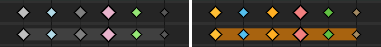
\includegraphics[width=0.45\textwidth]{blender_docs_images/keyframe_types.png}
    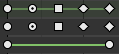
\includegraphics[width=0.3\textwidth]{blender_docs_images/animation_keyframes_introduction_interpolation.png}
    \caption{\textbf{To the left}, keyframe types. \textbf{To the right}, bezier interpolation handles type}
\end{figure}
\paragraph{Interpolation Mode Handles}
Similiarly to \textit{Keyframe Types}, the \textit{Dope Sheet Editor} shows Keyframe interpolation handles with \textit{Bezier} mode differently based on the handle type given in the F-Curve tab, 
giving us some visual feedback without having to open the \textit{Graph Editor}
\begin{itemize}[noitemsep, topsep=0pt]
    \item \textit{Circle}: Auto Clamped (default)
    \item \textit{Circle with Dot}: Automatic
    \item \textit{Square}: Vector
    \item \textit{Clipped Diamond}: Aligned
    \item \textit{Diamond}: Free
\end{itemize}
This holds only if the left handle and right handle have the same type, otherwise, it's always displayed as a Diamond.

\subsubsection{Keying Sets}
Reference Video: \href{https://www.youtube.com/watch?v=5g7EbDtlKGM}{https://www.youtube.com/watch?v=5g7EbDtlKGM}\\
Whenever you press \textbf{I} to create a keyframe, the newly created keyframw will automatically Store and therefore animate the whole \textit{Object Transform}, and animated properties 
appear grouped under the "Object Transform" group, or better, under the \textit{Keying Set} "CubeAction", .
\begin{center}
    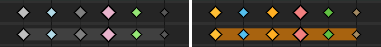
\includegraphics[width=0.5\textwidth]{blender_docs_images/keyframe_types.png}
\end{center}
If we want to animate only certain properties of our objects, we would need to spend time finding them in the appropriate tab inside the \textit{Properties Editor}, 
right click and "Insert Keyframe".\par
We can speed up the Keyframe creation process by specifying which properties we want to animate, and we can do that by creating a \textit{Keying Set}, found inside the \textit{Properties Editor}, under 
\mbox{"Scene/Keying Sets"}\footnote{Once you create a keying set, the default one won't be active anymore, and you need to add at least one property to the active (selected/highlighted)}.\par
Once you create a keying set, you can add properties to it by
\begin{enumerate}[noitemsep, topsep=0pt]
    \item Right Clicking the property (eg. from the \textit{Properties Editor}, Object Tab)
    \item Click "Add Single to Keying Set" to add the property to the active keying set
\end{enumerate}
Once you added it, go back to the \mbox{Scene/Keying Sets/Active Keying Set} panel and make sure that
\begin{itemize}[noitemsep, topsep=0pt]
    \item The \textit{Target ID Block}, ie to which object the keyframe should be applied has no object selected. This means that, regardless of which object you have selected, the keyframe will be 
      created from the object you specify here
    \item You can modify the \textit{Index} of the property, ie the order in which they appear inside the \textit{Dope Sheet Editor}
    \item You can modify how the animated properties are organized into a folder hierarchy by changing the \textit{F-Curve Grouping} (details in video)
\end{itemize}
Furthermore, if you want to export and import keying sets from a blender scene to another, you can click the \mbox{\textit{Export to File}} button to generate a Python script, which, executed on 
a new scene, will create the keying set you exported.\par\footnote{Maybe modifying that script you can also use the \texttt{bpy.context.active\_object} instead of fixing the keying set property object?}
Usage Limited on a specific scenario, for example
\begin{itemize}[topsep=0pt, noitemsep]
    \item You have a predefined set of objects you want to animate. Therefore, you can create a Keying set which encompasses all the properties across all the different objects you need
    \item You can select a frame, modify the properties of \textit{all the objects} to their desired value, and then press \textbf{I} once (instead of setting all the properties from the context 
    menu or pressing \textbf{I} for each object)
\end{itemize}
Instead of going to the \textit{Properties Editor}, \mbox{"Scene/Keying Sets"}, you can set the Active Keying set also from the \textit{Timeline Editor}, the Keying dropdown menu.

\subsection{Actions}
Video Reference: 
\begin{itemize}[noitemsep, topsep=0pt]
    \item Part1: \href{https://www.youtube.com/watch?v=x28RWgsIu8Y}{https://www.youtube.com/watch?v=x28RWgsIu8Y}\footnote{This rig is also available for download!}
    \item Part2: \href{https://www.youtube.com/watch?v=LXMiHvwIgDs}{https://www.youtube.com/watch?v=LXMiHvwIgDs}
\end{itemize}
Blender saves everything as a \textit{Data Block}, and animations are no exceptions. In fact, whenever we create a new keyframe, blender actually creates for us a new \textit{Action}, with a 
default name equal to \mbox{"(Object Name)Action"}. To visualize all Actions in your scene\footnote{Useful if you want to remove some unused data which is still present in the .blend file}
\begin{itemize}[noitemsep, topsep=0pt]
    \item In the \textit{Outliner Editor}, open the \textit{Data API} Display Mode, and click under the item "Actions"
\end{itemize}
The structure of the Action Data block is the following
\begin{center}
    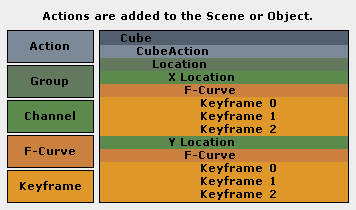
\includegraphics[width=0.5\textwidth]{blender_docs_images/animation_actions_data3.png}
\end{center}
Succinctly, \textbf{Actions are reusable animation segments}.\\
Actions can be managed from 2 places
\begin{itemize}[noitemsep, topsep=0pt]
    \item \textit{Dope Sheet Editor}, with Display Mode \textit{Action Editor} (and not the default \textit{Dope Sheet}, which gives an overview of the current action)
    \item \textit{NLA Editor} sidebar (See later \textit{Non Linear Animations})
\end{itemize}
This allow us to 
\begin{itemize}[noitemsep, topsep=0pt]
    \item Apply the same Action to different objects (as shown in the second video, in which the animation is first applied to a stand in, then applied to the final model)
    \item Store different animations applied to the same object (example running, walking, throwing a punch, ...), all starting from zero. Of course, we then need to \textbf{Combine} them together\\
    (Example: We want our character to run to a given position, and then throw a punch) (used with NLA)
\end{itemize}
In the \mbox{\textit{Dope Sheet Editor}/\textit{Action Editor}}, the Action Sidebar shows 2 checkboxes
\begin{itemize}[noitemsep, topsep=0pt]
    \item \textit{Manual Frame Range}: Instead of using the range specified by the \textit{Timeline Editor}, uses a manually specified frame range (used with NLA)
    \item \textit{Cyclic Animation} The animation is Cyclic over the specified range (used with the previous checkbox)
\end{itemize}
\paragraph{Non Linear Animations}
\begin{itemize}[noitemsep, topsep=0pt]
    \item Video Reference: \href{https://www.youtube.com/watch?v=Hz1TwvSNsrA}{https://www.youtube.com/watch?v=Hz1TwvSNsrA} (\textbf{Really Important})\\
    \item Blender Ref: \href{https://docs.blender.org/manual/en/4.3/editors/nla/introduction.html}{https://docs.blender.org/manual/en/4.3/editors/nla/introduction.html}
\end{itemize}
To combine different actions, we need to use the \textit{NLA Editor}. Brief description of the content of this editor
\begin{figure}
    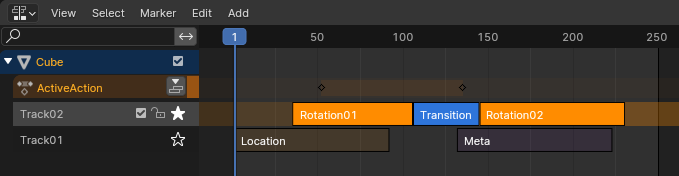
\includegraphics[width=0.5\textwidth]{blender_docs_images/editors_nla_tracks_example.png}
    \caption{Example of \textit{NLA Editor} Tracks}
\end{figure}
\begin{itemize}[noitemsep, topsep=0pt]
    \item Left Panel containing a down down menu for each object containing at least 1 action. Each dropdown menu is a \textbf{Stack of Actions}
    \item The Main Region displays a Stack of \textit{Track}, in which each Track is made up of \textit{Strips}. The top of the stack, highlighted in orange, which contains no strips, is the 
    object's \textit{Active Action}
    \item Right Panel, non empty only for the active object's action, having options \textit{Extrapolation} (already seen), \textit{Blending}, \textit{Influence}. Brief:
    \begin{itemize}[noitemsep, topsep=0pt]
        \item \textit{Blending}\footnote{Link: \href{https://docs.blender.org/manual/en/4.3/editors/nla/sidebar.html?utm_source=blender-4.3.2\#bpy-types-animdata-action-blend-type}{https://docs.blender.org/manual/en/4.3/editors/nla/sidebar.html?utm\_source=blender-4.3.2\#bpy-types-animdata-action-blend-type}}
          how to combine this action's property values with the ones from the track below (similiar to layer modes in Photoshop). Formulas used by each mode in the footnote link 
        \item \textit{Influence} how much the actions contributes to the NLA Stack
    \end{itemize}
\end{itemize}
Each Strip of an NLA Track has 2 fundamental settings 
\begin{itemize}[noitemsep, topsep=0pt]
    \item \textit{Extrapolation} should we hold the pose once the strip finishes?
    \item \textit{Blending} how to mix with NLA tracks underneath
    \item \textit{Blend In} and \textit{Blend Out} Fade effects for when the strip starts and finishes playing
\end{itemize}
\begin{mdframed}[linewidth=2pt, linecolor=gray, roundcorner=1pt, innermargin=2pt, outermargin=2pt]
    \textbf{\Large Quick Experiment: Actions and Non Linear Animation: "Enlarge and Shoot"} \\[6pt]
    \textbf{File:} \texttt{03\_Actions\_NLA-Cube\_Path.blend} \\[6pt]

    \begin{enumerate}[topsep=0pt, noitemsep]
        \item Create a Cube, and in the \mbox{\textit{Dope Sheet Editor}/\textit{Action Editor}} create a new Action, call it \mbox{"Cube\_Enlarge"}
        \item Open the \textit{NLA Editor} alongside \mbox{\textit{Dope Sheet Editor}/\textit{Action Editor}}, and \textit{Push Down} (either from NLA Editor of from Dope Sheet) the current action.\\
        As you can see, this will create a new \textit{Track} containing a single \textit{Strip} which contains the action we just pushed.
        \begin{itemize}[noitemsep, topsep=0pt]
            \item Now the object has no active action, and in fact the dope sheet is empty...
            \item ... But if you press \textbf{Shift + Left Arrow} and \textbf{Spacebar} (go to beginning of timeline and play), the animation still plays out, because the final animation is the 
              \textbf{composition of the whole NLA Stack}
            \item On the newly created \textit{Track}, try to grab the \textit{Strip} and move it along the Track's timeline. A strip can be placed wherever we want in the frame range
            \item To the left of each \textit{Track} there is a visibility checkbox. If deactivated, the \textit{Track}'s animation won't be played out
        \end{itemize}
        \item Create another action to move the cube, with an "explosive" F-Curve, ie most of the displacement is done earlier in the F-Curve (therefore you need to open it in the \textit{Graph Editor})\\
          (it is reccomended to turn off all NLA Tracks while working on another action in the \textit{Dope Sheet})
        \item Push down the newly created Action in the NLA Stack. This will create a new NLA Track. We don't want that, so click and drag the \textit{Strip} in the new \textit{Track} onto the 
        existing track, delete the now empty track, and place the Shoot Action after the Enlarge action. The result should be something like this:
        \begin{center}
            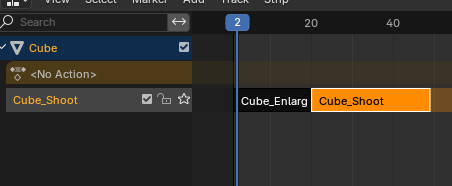
\includegraphics[width=0.5\textwidth]{blender_docs_images/my_nla_example.png}
        \end{center}
        \item Note: \textbf{Having more strips that modify different properties will reset all the work done by the previous strip, even if Extrapolation is set to Hold in the right side panel, strip menu}\\
            As you can see playing out the animation, after the Enlarge Action is done, the cube snaps back to its original scale and starts traslating. Fix:
            \begin{itemize}[noitemsep, topsep=0pt]
                \item Have \textit{Strips} which modify different properties in different \textit{Track}s. Therefore, from the topbar of the Editor, with a track selected, Click \mbox{Track/Add} and 
                    move one of the two strips in the newly created Track\footnote{Remember to rename the tracks in a "serious" project}
            \end{itemize}
    \end{enumerate}
    {\tiny Quick Tip: In your Animation Layout, use two bottom panels, the bottom one \textit{NLA Editor}, and the top one will switch between \mbox{\textit{Dope Sheet Editor}/\textit{Action Editor}}
      and \textit{Graph Editor} with the shortcuts \mbox{\textbf{Shift + F12}} and \mbox{\textbf{Shift + F6}}
    }
\end{mdframed}
Important Note: \textbf{Unassigned Actions are LOST when you quit blender if they are not used by anybody, therefore you need to protect them with a fake user}.\\
As a remainder on how to add a fake user, you can do it in different ways, one of them is by clicking the "Shield" icon from the \mbox{\textit{Outliner Editor}/Blender File} Display mode, under Actions.\par
For more detail, eg how to \textit{Repeat} (Under \mbox{NLA Editor/Strip/Action Clip/Repeat}) a Strip, check out the Reference video.

\subsection{Armatures}
\begin{itemize}[noitemsep, topsep=0pt]
    \item Video Workshop: \href{https://www.youtube.com/watch?v=iZBLtooU2Cs}{https://www.youtube.com/watch?v=iZBLtooU2Cs} (This is a follow along type of tutorial. from beginning to 58:51 is about armature creation, then follows skinning, then in 1:22:01 armature keyframed animation)
    \item Blender Docs: \href{https://docs.blender.org/manual/en/4.3/animation/armatures/introduction.html}{https://docs.blender.org/manual/en/4.3/animation/armatures/introduction.html}
    \item Reference Rig: \href{https://blendswap.com/blend/25094}{https://blendswap.com/blend/25094}
    \item Note: Use Quaternion as rotation mode
\end{itemize}
An \textit{Armature} is a hirerachical structure of \textit{Bones} (an Acyclic Directed Graph, to be precise).\par
To create a bone in a fresh blender scene, use \mbox{Add/Armature}. Observe in the \mbox{\textit{Outliner Editor}}, \textit{Blender File} Display mode, what a bone created for us.
\begin{enumerate}[noitemsep, topsep=0pt]
    \item Expand the \textit{Armatures} tab and \textit{Objects} tab.
    \item As you can see, we created an \textit{Armature}, and an Object containing that armature.
    \item The armature has inside it a composite structure
    \begin{itemize}[noitemsep, topsep=0pt]
        \item \textit{Pose} The object itself has an additional data property, which is the Pose (in fact, there is a Armature tab in the \textit{Properties Editor})
        \item \textit{Bone} Hierarchy and \textit{Bone Collection} inside the armature
        \item Go to edit mode and extrude the bone. Now the bone hierarchy has an additional bone
    \end{itemize}
\end{enumerate}
Once you select an armature object, you can see from the viewport that it has only 3 modes: \mbox{Object Mode}, \mbox{Edit Mode}, and \mbox{\textit{Pose Mode}}
\begin{itemize}[noitemsep, topsep=0pt]
    \item Edit Mode: Create More bones
    \item Pose Mode: The Armature is done, and you want to create some key poses for your armature
\end{itemize}
To have X-Ray on the bones, click, inside the Data tab in the \textit{Properties Editor} the option \mbox{\textit{Viewport Display/In Front}}.\\
To Rename your selected bone, use \textbf{F2}.\\
If the armature is supposed to be symmetric
\begin{figure}
    \centering
    \label{symm::armature}
    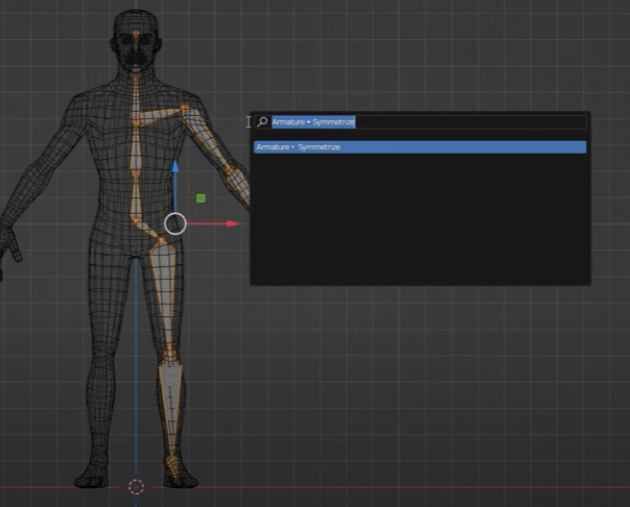
\includegraphics[width=0.5\textwidth]{blender_docs_images/my_symmetric_armature.png}
    \caption{Symmetrizing an Armature}
\end{figure}
\begin{itemize}[noitemsep, topsep=0pt]
    \item Create one side (eg right arm, right leg) and the middle too
    \item Click \textbf{F3} and type "Armature Symmetrize" (See figure \ref{symm::armature})
    \item \textbf{Symmetrization works only if you follow the blender naming conventions with blender}. Renaming bones therefore becomes mandatory\\
    There are different variants, basically you have to use the format "\textit{Thing\_R}" for right and "\textit{Thing\_L}" for left, and no suffix for bones in the middle.\\
    Link: \href{https://docs.blender.org/manual/en/4.3/animation/armatures/bones/editing/naming.html\#armature-editing-naming-conventions}{https://docs.blender.org/manual/en/4.3/animation/armatures/bones/editing/naming.html\#armature-editing-naming-conventions}
\end{itemize}
To visualize the hierarchy of bones without using the Outliner, you can use the \mbox{\textit{Properties Editor}}, in the \textit{Bones} Data tab, under "Relations", in which you can see the direct
parent of the selected bone.\par
To create a new bone, you can Extrude it with \textbf{E} in Edit mode, but you can also use the \textit{Subdivide} command from the edit mode context menu (with a bone selected).

\paragraph{Forward Kinematic vs Inverse Kinematic}
If you create a bone hierarchy, go to \mbox{\textit{Pose Mode}}, and then try to move one of its bones (example: a hand of a humanoid character), you'll notice that you can only rotate the selected bone
subtree. By default, by moving a bone, you \textbf{move only its subtree}, ie \textbf{a child cannot move a parent}.\par
What if we want to move the hand of our humanoid and we want the elbow to follow it? \textit{Inverse Kinematic}\par\footnote{Side: To clear the pose in \textit{Pose Mode}, use \mbox{"Pose/Clear Transform/All"}}
To create an \textit{IK Rig} (Workshop video, 26:16), we need
\begin{itemize}[noitemsep, topsep=0pt]
    \item \textbf{create \textit{IK Target}}, which is a duplicate bone (\textbf{Shift + D}) of the bone that should trigger inverse kinematic (eg hand, foot)\footnote{Naming convention: OriginalBoneName + IK + \_L/\_R}
    \item with the duplicate bone selected, go to \textit{Properties Editor}, Bones Data Tab, "Relations" and \textbf{remove the parent}
    \item Press \textbf{N} (Edit Mode) and adjust the Length property of this bone, such that it is easier to select
    \item Before adding any IK constraints, once your basic bones are already placed, \textbf{reset all bones roll}: \mbox{Armature/Bone Roll/Recalculate Roll/View Axis} (from a character-frontal orthographic view)
    \item Go back to \textit{Pose Mode}, select the bones you need to affect and go to the \textit{Bone Constraint} tab, add the constraint \textit{Inverse Kinematic}. Under its options
    \begin{itemize}[noitemsep, topsep=0pt]
        \item Select as target: the armature itself
        \item select as bone: IK Bone\footnote{At this point, IK works, but the IK target moves the whole armature}
        \item Select the bone with the constraint and change the \textit{Chain Length} property (0 = infinite, 1 = affect only 1 adjacent bone)\footnote{At this point, the original bone doesn't follow the orientation of the IK bone}
        \item select the original bone, and add a bone constraint \textit{Copy Rotation}, and set the Target Property: armature, and Bone: IK Bone\footnote{The IK Bone can still move freely, don't make it go too far}
        \item with the IK Bone selected, go to the bone data tab and check off the tab \textit{Deform}.\footnote{we don't want the IK bones to pull vertices of the mesh once skinned}
    \end{itemize}
\end{itemize}
After you've done that, say you want to hide the original hand bone (since you'll be manipulating the IK one), you can do that by moving the hand bone into a different \textit{Bone Layer}. Bone layer
options can be found under the \textit{Armature} data tab in \mbox{\textit{Properties Editor}}, "Skeletor/Layers", or you can select the bone and press \textbf{M}. Then, you can turn on/off bone layers
as you need.

\paragraph{IK Pull Target}
(Video Workshop: 35:16)\\
Say you want to realize an elbow for a humanoid character. When animating it, you don't want to manipulate the forearm directly, you want to control a handle which should be the direction into which the 
elbow tip should point to, ie, a \textit{Pull Target}.\footnote{process used for knee, elbow, ...}
\begin{itemize}[noitemsep, topsep=0pt]
    \item With the elbow \textbf{Joint}\footnote{joint = little sphere, bone = connects two joints} selected, extrude a new bone strictly backward.\footnote{to a position in which the elbow cannot reach} (call that ElbowIK\_L)
    \item Remove the parent of the newly selected bone (Relations tab under the bone data tab in the \mbox{\textit{Properties Editor}})
    \item Select the forearm bone (the one whose base joint contains is elbow), go in \textit{Pose Mode}, which should already have an IK constraint (if you configured the hand), 
    select as \textit{Pull Target} the armature itself, and as \textit{Bone} for the pull the elbow IK bone.
    \item Change the \textit{Pole Angle} in the IK Constraint such that it matches the desired direction (it's a trial and error process, so move around the forearm)
\end{itemize}

\paragraph{Controller Bone}
A Bone to move the whole character:
\begin{itemize}[noitemsep, topsep=0pt]
    \item move the 3D Cursor where the bone controller should be (eg. world origin)
    \item Create a new armature object. The newly created bone will be the new parent of the other armature object
    \item Turn off deform for this controller bone (Bone Data tab inside the \mbox{\textit{Properties Editor}})
    \item therefore select first then the original armature the controller and press \mbox{\textbf{Ctrl + P}} (\mbox{Control Parent}) and click \mbox{\textit{Keep Offset}}\footnote{now the IK Bones are not following the controller}
    \item select all IK Bones (ie bones which are not in the hierarchy), then select the controller bone and \mbox{\textbf{Ctrl + P}}
\end{itemize}

\paragraph{Non Limb Bones}
We are referring to bones which should animate part of a model which is separated (on a different mesh object) (example: Hen Welding Helmet). While you can modify its pivot and keyframe its rotation, 
having a bone with some predefined poses makes the whole process much easier.\par
These bones, \textbf{even if they affect a different mesh the armature is a single hierarchy}, so use \mbox{\textbf{Ctrl + P}} after placing your bone. Furthermore, all of these bones should have 
\textit{Deform} (from the bone data tab in the \mbox{\textit{Properties Editor}}) turned off, such that they do not influence the main body\footnote{How to skin and influence different parts later}. That's
because the non-limb parts just need to rotate following the bones, not deform.\par
When skinning with non limb bones, use parenting with \textit{Bone}, and not \textit{Armature Deform}, \textbf{With the correct bone selected}

\paragraph{Bones Viewport display}
Changes the way bones are visualized (some can be manipulated in edit mode by scaling bones (remember to reset transform)). Viewport Display is found in the \textit{Armature} Data Tab in the
\mbox{\textit{Properties Editor}}

\subsection{Skinning and Topology}
Here are some links:
\begin{itemize}[noitemsep, topsep=0pt]
    \item Topology Guide: \href{https://topologyguides.com/}{https://topologyguides.com/}
    \item Retopology in blender: \href{https://www.youtube.com/watch?v=1myOZaxtHes}{https://www.youtube.com/watch?v=1myOZaxtHes}
    \item Topology for animation video: \href{https://www.youtube.com/watch?v=qfSRiE-6FtA}{https://www.youtube.com/watch?v=qfSRiE-6FtA}
\end{itemize}

\subsubsection{Bones}
As we've seen, bones can be classified into 2 basic categories, \textit{Deforming Bones} and \textit{Control Bones}
\begin{itemize}[noitemsep, topsep=0pt]
    \item \textit{Deforming Bones}: Bones which, when transformed, will transform the vertices they are associated with (See Section \ref{armature:skinning})
    \item \textit{Control Bones}: They control other bones and have no direct effect on vertices. Examples of this are \textit{IK Target Bones} and \textit{Main Controller Bone}
\end{itemize}

\paragraph{Bone Collections}
Similiarly to how you can group objects into Collections in the \mbox{\textit{Outliner Editor}}, you can group bones into \mbox{\textit{Bones Collections}}. \textbf{This won't affect the bones hierarchy}.
Bone Collections can be created and managed from the \textit{Armature} and \textit{Bone} Property Panels in the \mbox{\textit{Property Editor}}.\par\footnote{Note: Bone Collections are a blender 4.0 
replacement for armature layers and bone groups}
There are 2 primary usages for Bone Collections:
\begin{itemize}[noitemsep, topsep=0pt]
    \item \textbf{Organization and visibility}: You can turn off each layer group individually
    \item \textbf{Library Overrides}\footnotemark: When you try to \textit{Link} an armature\footnote{Meaning The Armature Itself + Armature Object}, you can modify the imported bone collections by
    \begin{enumerate}[noitemsep, topsep=0pt]
        \item Link The Armature, which should be inside a collection. \mbox{\textit{File/Link}}.
        \item Select the linked armature and go to \mbox{\textit{Object/Relations/Make Library Override}} (\mbox{\textbf{Ctrl + Shift + O}})
        \item In \mbox{\textit{Pose Mode}}, open the \textit{Bone Collections} panel in the Armature Properties tab
        \item Click the \textit{Override} Button (Outliner, Right click on the component with the chain icon, select \mbox{\textit{ID Data/Make Library Override Hierarchy}})
        \item Change the link mode for the bone collections from data to object (see video footnote, minute 5:00 - 5:15)
        \item (Maybe?) \textbf{Ctrl + L} and check the appropriate link option
    \end{enumerate}
    \footnotetext{Link on Library overrides: \href{https://www.youtube.com/watch?v=nujaW-qNoRk}{https://www.youtube.com/watch?v=nujaW-qNoRk}}
\end{itemize}
Bone Collections Example:
\begin{itemize}[noitemsep, topsep=0pt]
    \item FK Controls
    \item IK Controls
    \item Face Controls
    \item Face Detail Controls
\end{itemize}

\paragraph{Bone Selection Shortcuts}
Reference: \href{https://docs.blender.org/manual/en/4.3/animation/armatures/bones/selecting.html}{https://docs.blender.org/manual/en/4.3/animation/armatures/bones/selecting.html}
\begin{longtable}{lp{0.7\textwidth}}
    \toprule
    \textbf{Shortcut} & \textbf{Brief} \\
    \midrule
    \endhead
    \midrule
    \multicolumn{2}{r}{Continue...} \\
    \bottomrule
    \endfoot
    \bottomrule
    \endlastfoot

    \textbf{[}, \textbf{]} & Select Parent, Select Child \\
    \textbf{Shift + [}, \textbf{Shift + ]} & Extend selection with Parent, Extend Selection with Child \\
\end{longtable}

\paragraph{Bone Editing}
Very similiar to Mesh Editing. We've already seen how \textit{Extrude}, \textit{Subdivide}, \textit{Grab}, \textit{Symmetrize}, \textit{Parenting}, \textit{Naming} work in the first paragraph of this
subsection. you can find additional commands, such as \textit{Split} (\textbf{P}), in the documentation \href{https://docs.blender.org/manual/en/4.3/animation/armatures/bones/editing/index.html}{https://docs.blender.org/manual/en/4.3/animation/armatures/bones/editing/index.html}.\par
An important editing command, which should be performed before skinning, is \textit{Bone Roll Recalculation} (\mbox{\textit{Armature/Bone Roll/Recalculate Roll}} or \textbf{Shift + N})

\paragraph{Bone Properties}\footnote{Excluding Transform, Viewport Display, Relations, which have been already covered}
\begin{itemize}[topsep=0pt, noitemsep]
    \item \mbox{\textit{\textbf{Bendy Bones}}} Bones which can be curved, as they are represented as a Bezier Curve. Perfect for modeling chains of small ligaments/bones such as the Human spine column or
    facial bones. In Edit Mode, we can control the Bendy Bone as a Bezier Curve, and its properties editor, under the bendi bone panel, has your typical Bezier Curve Controls, such as number 
    of \textit{Segments}, Reference: \href{https://docs.blender.org/manual/en/4.3/animation/armatures/bones/properties/bendy_bones.html}{https://docs.blender.org/manual/en/4.3/animation/armatures/bones/properties/bendy\_bones.html}
    \item \mbox{\textit{\textbf{Inverse Kinematics}}} Controls how the bone behaves when linked in a \textbf{Inverse Kinematic Chain}\footnote{Signaled with a yellow line}. More details on this in the 
    Posing SubSection, Bone Constraints Paragraph
    \item \mbox{\textit{\textbf{Deform}}} Checks whether the bone should deform the parented mesh\footnote{Through the Armature Deform Tool with Automatic Weights} or not. The bone defines a volume of 
    space inside which vertices are affected. Such volume is called \textit{Envelope}. We can control its Size with \mbox{\textit{Envelope Distance}}, Head and Tail Radius. \textbf{Envelopes are 
    considered only if you skin with \mbox{Deform/With Envelope Weights}}
    \begin{center}
        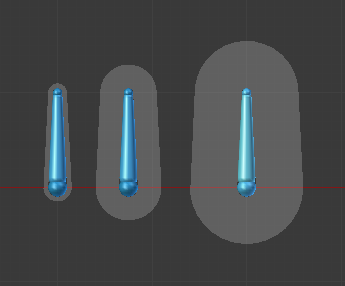
\includegraphics[width=0.3\textwidth]{blender_docs_images/animation_armatures_bones_properties_deform_envelope-distance.png}
    \end{center}
    Furthermore, for parts of the geometry shared by more than 1 bone, we can use the \textit{Envelope Weight} option on these neighboring bones to given an importance to each.
\end{itemize}

\subsubsection{Armature Properties}
Basic ones:
\begin{itemize}[noitemsep, topsep=0pt]
    \item Pose tab to switch between the rest position of the armature and the current pose position
    \item Motion Paths (See Motion Path Animation Subsection)
    \item Inverse Kinematic: chooses the IK Solver (See Bone Constraints paragrah, Inverse kinematic)
    \item Bones Collection (Explained above)
\end{itemize}

\subsubsection{Skinning}\label{armature:skinning}
Select the mesh, select the armature\footnote{child then parent}, \mbox{\textbf{Ctrl + P}} -> Choose \mbox{Armature Deform/With Automatic Weights}. The mesh not has a \textit{Armature} Modifier\footnote{Be 
carefor of where in the modifier list the armature modifier is. Exmaple: It shouldn't be on below a subdivision modifier, such that it controls a simpler mesh. It shouldn't be above a mirror modifier, 
otherwise only the original mesh, and not the mirrored one, will be deformed. \textbf{Modifiers are applied top to bottom}}\par
The mesh, skinned with automatic weights, never works properly. We need to use the \textit{Weight Paint Mode} to manually adjust the weights of each bone.\par
To check the vertex weights for a given vertex
\begin{enumerate}[noitemsep, topsep=0pt]
    \item Select a skinned mesh and go to \mbox{\textit{Edit Mode}}, select a vertex
    \item press \textbf{N} to bring up the sidebar, select the \textit{Item} tab and expand the \mbox{\textit{Vertex Weights}} submenu. This will contain a list of bones which have a nonzero weight
\end{enumerate}
In fact, once you skinned with automatic weights, blender created for you a \mbox{\textit{Vertex Group}} for each bone (with the same name). Each \mbox{\textit{Vertex Group}} contains the vertices that 
are affected by a given bone.
\begin{itemize}[noitemsep, topsep=0pt]
    \item with the skinned mesh selected, go to the Data panel of the \mbox{\textit{Properties Editor}}, \mbox{\textit{Vertex Group}} and select a vertex group for a bone. Pressing \textbf{A} with a 
    vertex group selected will select all vertices in the vertex group
\end{itemize}
From the above considerations, we understand that blender has Two ways of Skinning
\begin{itemize}[topsep=0pt, noitemsep]
    \item \mbox{\textit{\textbf{Parent/Constrain Objects to Bones}}}: When you transform the bones in \mbox{\textit{Pose Mode}}, the "Child" mesh gets transform bot \textbf{never} deformed
    \item \mbox{\textit{\textbf{Armature Modifier on a mesh}}}\footnote{WHat the \mbox{Armature Deform/With Automatic weights} does}: Deform the geometry of the objects based on per bone weight 
    association to some vertex groups
\end{itemize}

\paragraph{Weight Paint Overview}
Video Workshop: 1:14:25\\
Clicking \mbox{\textbf{Ctrl + RMB}}\footnote{I use right mouse button selection, otherwise left mouse button} lets you select the bone you want to edits the weights of.\\
By clicking into the brush icon (under the \mbox{"Weight Paint"} text) you can select the type of brush you want to use. By type we mean the math operation done to the weights. (eg. add, subtract).\\
In weight painting, having a \textbf{mirror modifier} saves you a lot of headache! Blender can recognize .R and .L bones with the mirror modifier!\\
In short, follow this simple 6 step guide: \href{https://docs.blender.org/manual/en/4.3/sculpt_paint/weight_paint/usage.html}{https://docs.blender.org/manual/en/4.3/sculpt\_paint/weight\_paint/usage.html}

\subsubsection{Posing}
\begin{itemize}[topsep=0pt, noitemsep]
    \item Docs Reference: \href{https://docs.blender.org/manual/en/4.3/animation/armatures/posing/introduction.html}{https://docs.blender.org/manual/en/4.3/animation/armatures/posing/introduction.html}
    \item Video Reference: 
    \item Pose Library: \href{https://www.youtube.com/watch?v=95rcqlpsMO4}{https://www.youtube.com/watch?v=95rcqlpsMO4}
    \item Pose to Pose Workflow\footnote{Watch This when you already know the basics}: \href{https://www.youtube.com/watch?v=p8Bi7k60IS0}{https://www.youtube.com/watch?v=p8Bi7k60IS0}
\end{itemize}
Once an Armature is skinned to some objects and ready to go, we need to configure particular armature (or part of it) positions into \textit{Poses} (Example: 
clenched fist Pose, which edits only the finger bones).\par
The main course here is to use \textit{Pose Mode}. Its selection commands are the same of Edit Mode, plus \mbox{\textit{Select/Constraint Target}} which selects the bones used as target by the currently
selected bones.\\
If, during editing of a particularly heavy Skinned object, you experience some lag, you can enable, in the \mbox{\textit{Armature Panel}}, the \mbox{\textit{Delay Deform}} button, which will trigger the 
deformation only when you finish transforming a bone.\\
For a thorough overview of \textit{Pose Mode}, let us exclude commands analogous to \textit{Edit Mode} like \textit{Apply} or \textit{Clear Transform}.
\begin{itemize}[topsep=0pt, noitemsep]
    \item \textit{Copy Paste} in Pose Mode, will actually copy the pose of the selected bones. Also, if you want to flip the pose along the X axis, you can use \mbox{\textit{Paste Flipped}} (\mbox{\textbf{Ctrl + Shift + V}})
    \item \textit{Propagate} (\mbox{\textbf{Alt + P}}) the current pose to another Keyframe/keyframe range (specified in options like "To Next Keyframe")
    \item \mbox{\textit{In-Between Tools}}: Tools to control interpolation between poses. All the following commands are in the \mbox{\textit{Pose/In-Betweens/}} menu, and some have shortcuts
    \begin{itemize}[noitemsep]
        \item \mbox{\textbf{\textit{Push Pose From Breakdown}}} (\mbox{\textbf{Ctrl + E}}) interpolates the current pose by making it closer to the next keyframed position. 
        Video Reference: \href{https://www.youtube.com/watch?v=R0o_yHwSafE}{https://www.youtube.com/watch?v=R0o\_yHwSafE} (first 3 minutes).\\ Similiar is \mbox{\textit{Pose Breakdowner Tool}}, which does 
        the same thing, but it is interactive and therefore gives more control. For example, we can choose (like the Grab tool) which "axes" to affect
        \begin{itemize}[topsep=0pt, noitemsep]
            \item \textbf{G, R, S}: move, rotate, scale
            \item \textbf{X, Y, Z}: to the corresponding axes
            \item \textbf{B}: Bendy bones
        \end{itemize}
        \item \mbox{\textbf{\textit{Relax Pose To Breakdown}}}\footnotemark while the previous tools brings the pose closer to the next keyframe, this one pulls the pose closer to the previous keyframed position
    \end{itemize}
\end{itemize}
\footnotetext{There are also push/relax pose with respect to the rest pose}

\paragraph{Pose Library}
To bring together Armatures with a Skinned Mesh, Actions, and the NLA Editor, the \textbf{\textit{Pose Library}} comes into play. It is a simple .blend file which will store a catalogue of poses for a 
given object, each stored as a so-called \textit{\textbf{Pose Asset}}.\par
First and foremost, a brief introduction on the \textit{Asset Browser} (\small Video Reference: \href{https://www.youtube.com/watch?v=cbzBt60dhY8}{https://www.youtube.com/watch?v=cbzBt60dhY8}).\par

\paragraph{Bone Constraints: Inverse Kinematics}
Inverse Kinematics is a bone-based posing technique which allows \textbf{automatic positioning of a Chain of bones} by only manipulating the \textbf{Last bone in the chain}. (see example in introduction to armatures).\par
Such Constraints are \textit{\textbf{IK Solver}} and \textit{\textbf{Spline IK}}, which will be discussed when talking about Tracking in Subsection \ref{constraints}. In here, instead, we discuss the 
bone panel properties about \textit{Inverse Kinematic}, for the standard solver
\begin{itemize}[topsep=0pt, noitemsep]
    \item \textit{IK Stretch} Stretch influence to IK target.
    \item \textit{Lock} Disallow movement around the axis.
    \item \textit{Stiffness} Stiffness around the axis. Influence disabled if using Lock.
    \item \textit{Limit} Limit movement around the axis.
\end{itemize}
While \textit{IK Solver} tries to align a chain to point towards a Target and flex with respect to a Pull Target, the \textit{Spline IK} is a constraint which aligns  a chain of notes along a curve.
Useful to model Tentacles, Tails, Ropes, ...\par
To setup Spline IK, it is necessary to have a chain of connected bones and a curve to constrain these bones to:
\begin{enumerate}[topsep=0pt, noitemsep]
    \item With the last bone in the chain selected, add a Spline IK Constraint from the Bone Constraints tab in the Properties.
    \item Set the Chain Length setting to the number of bones in the chain (starting from and including the selected bone) that should be influenced by the curve.
    \item Finally, set the Target field to the curve that should control the curve.
\end{enumerate}
Tips:
\begin{itemize}[noitemsep, topsep=0pt]
    \item not too long bones and with same length
    \item Use few control points
\end{itemize}
Complete controls in \url{https://docs.blender.org/manual/en/4.3/animation/armatures/posing/bone_constraints/inverse_kinematics/spline_ik.html}\\
Video reference in \url{https://www.youtube.com/watch?v=vZaNZhAoMts}

\subsection{Constraints}\label{constraints}
\begin{center}
    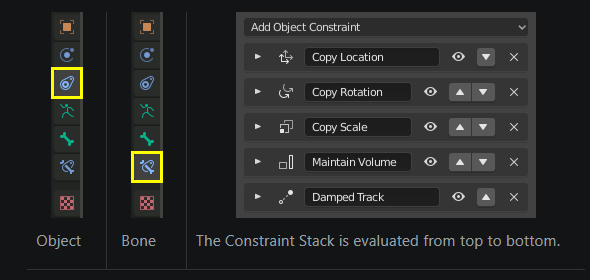
\includegraphics[width=0.5\textwidth]{blender_docs_images/my_constraint_stack.png}
\end{center}

\subsection{Lattice}
3D Grid created with the \textit{Lattice Modifier}. It is basically a localized Proportional Editing used to deform a mesh, mainly to create \textit{Shape Keys} (See subsection \ref{shapekeys})

\subsection{Drivers}
\begin{enumerate}[noitemsep, topsep=0pt]
    \item Intro: \href{https://www.youtube.com/watch?v=rdHIrK6qvxM}{https://www.youtube.com/watch?v=rdHIrK6qvxM}
\end{enumerate}
A driver is a relationship tool which controls the properties of some objects with properties of some other objects, as specified by a function\footnote{Namely, an F-Curve} or mathematical expression.\par
The languages the driver mathematical expressions use is a subset of the Python Programming language. Quick Reference: \url{https://docs.blender.org/manual/en/4.3/animation/drivers/drivers_panel.html#drivers-simple-expressions}\par
\paragraph{Introduction Workflow from video}
To create a Driver from a property, right click on it and \mbox{\textit{Copy as a new Driver}}. This will put it into the clipboard, therefore you can go into another property of another object and 
use \mbox{\textit{Paste Driver}}. \textbf{The drived property becomes purple}.\\
Of course, once a driver is created, it is visible from the \textit{Outliner} in \textit{Blender File} Display Mode.\par
As a metaphor, Blender Drivers are very similiar to Excel Sheet's computed cell values.\\
Another button is: Right click to a property and \mbox{\textit{Add A Driver}}, which will open an Expression editor
\begin{wrapfigure}{l}{0.25\textwidth}
    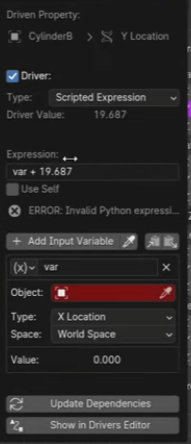
\includegraphics[width=0.2\textwidth]{blender_docs_images/my_driver_scriptable_expression.png}
    \caption{Scriptable Expression editor after \textit{Add A Driver}}
\end{wrapfigure}
Once you close that popup, you need to Open the \textit{Driver Editor} and select the object with driven (purple) properties to get it back.

\subsection{Shape Keys}\label{shapekeys}

\subsection{Motion Paths}

\section{Animations Through Physics}
https://www.youtube.com/watch?v=69peFKU4XqI

\section{Compositing Essentials}

\section{Video Editing Essentials}

\end{document}
